
% 
% Annual Cognitive Science Conference
% Sample LaTeX Paper -- Proceedings Format
% 

% Original : Ashwin Ram (ashwin@cc.gatech.edu)       04/01/1994
% Modified : Johanna Moore (jmoore@cs.pitt.edu)      03/17/1995
% Modified : David Noelle (noelle@ucsd.edu)          03/15/1996
% Modified : Pat Langley (langley@cs.stanford.edu)   01/26/1997
% Latex2e corrections by Ramin Charles Nakisa        01/28/1997 
% Modified : Tina Eliassi-Rad (eliassi@cs.wisc.edu)  01/31/1998
% Modified : Trisha Yannuzzi (trisha@ircs.upenn.edu) 12/28/1999 (in process)
% Modified : Mary Ellen Foster (M.E.Foster@ed.ac.uk) 12/11/2000
% Modified : Ken Forbus                              01/23/2004
% Modified : Eli M. Silk (esilk@pitt.edu)            05/24/2005
% Modified : Niels Taatgen (taatgen@cmu.edu)         10/24/2006
% Modified : David Noelle (dnoelle@ucmerced.edu)     11/19/2014

%% Change ''letterpaper'' in the following line to ''a4paper'' if you must.

\documentclass[10pt,letterpaper]{article}

\usepackage{cogsci}
\usepackage{pslatex}
\usepackage{apacite}
\usepackage{amsmath,amssymb}
\usepackage{graphicx}
\usepackage{color}
\usepackage{url}
\usepackage{todonotes}
\usepackage{mathtools}
\usepackage{stmaryrd}
\usepackage{booktabs}

\newcommand{\den}[2][]{
\(
\left\llbracket\;\text{#2}\;\right\rrbracket^{#1}
\)
}

%\newcommand{\url}[1]{$#1$}

\definecolor{Blue}{RGB}{0,0,255}
\definecolor{Red}{RGB}{255,0,0}
\newcommand{\red}[1]{\textcolor{Red}{#1}}
\definecolor{Green}{RGB}{10,200,100}
\newcommand{\ndg}[1]{\textcolor{Green}{[ndg: #1]}}
\newcommand{\jd}[1]{\textcolor{Blue}{[jd: #1]}}  

 \newcommand{\denote}[1]{\mbox{ $[\![ #1 ]\!]$}}


\newcommand{\subsubsubsection}[1]{{\em #1}}
\newcommand{\eref}[1]{(\ref{#1})}
\newcommand{\tableref}[1]{Table \ref{#1}}
\newcommand{\figref}[1]{Figure \ref{#1}}
\newcommand{\appref}[1]{Appendix \ref{#1}}
\newcommand{\sectionref}[1]{Section \ref{#1}}

\title{Animal, dog, or dalmatian? Level of abstraction in nominal referring expressions}
%Animal, dog, or dalmatian? Contextual informativeness, utterance length and utterance frequency affect choice of referring expressions.

 
\author{{\large \bf Caroline Graf, Judith Degen, Robert X.D. Hawkins, Noah D.~Goodman} \\
  cgraf@uos.de, \{jdegen,rxdh,ngoodman\}@stanford.edu\\
  Department of Psychology, 450 Serra Mall \\
  Stanford, CA 94305 USA}



\begin{document}

\maketitle


\begin{abstract}

\red{The choice of referring expressions is highly context dependent. Whether speakers choose to refer to an object as a ``dalmatian'', a ``dog'', or an ``animal'' is determined partly by the features of the other objects present in the scene, as well as features of the utterance alternatives. In the first step, an exploratory analysis within a reference game setting demonstrates that speakers' choice of referring expression is dependent on a rich interplay of expressions' degree of contextual informativeness, their relative length combined with their relative frequency, as well as on the degree to which the referent is typical of a specific expression. If a competitor object of the same category (e.g., dog) as the target object is present in the display, speakers choose a more specific subcategory (e.g., ``dalmatian'') to refer to the target object. In contrast, when the competitor objects do not share the same (super-) category as the target, speakers are less constrained in choosing an appropriate referring expression. In this event, shorter expressions are preferred over longer ones, even more so when frequency of the expression is high. Moreover, the better the referent fits to the meaning of a referential expression due to being more typical of it, the more this expression is preferred. In a second step, quantitative effects are analyzed by a production model couched in the Rational Speech Act framework, which predicts the pattern of results by modelling a speaker as balancing an utterance's contextual informativeness with its cost relative to its alternatives while taking into account soft semantics of the meanings of expressions due to typicality effects.}

\textbf{Keywords:} 
referential expressions, levels of reference, overinformativeness, basic levels, categorization
\end{abstract}

\section{\bf Introduction}

%Reference is ubiquitous in human communication. Unsurprisingly, a wealth of literature has been devoted to how speakers choose referring expressions from the many options available to them with the goal of distinguishing one object from its surroundings \red{cite cite cite deutsch pechmann sedivy gatt}. 
Referring to objects is a core function of human language, and a wealth of research has explored how speakers choose referring expressions \red{cite cite cite deutsch pechmann sedivy gatt}. 
However, most of this literature has focussed on the addition of modifiers (as in the choice between ``the dog'', ``the brown dog'', and ``the big brown dog''). Here we investigate how speakers choose a simple nominal referring expression---what governs the choice of calling a particular object ``the dalmatian'', ``the dog'', or ``the animal''? 
Noun choice can be seen as the most basic decision in forming a referring expression.
Like modification, these choices differ in their specificity; unlike modification, the number of words used does not differ---\emph{some} noun must be chosen.
In this paper we provide experimental evidence from a coordination game regarding the flexible choice of nominal referring expressions and explain this data with a probabilistic model of pragmatics.

%they differs in that
%Given the taxonomic relations that hold between dalmatians, dogs, and animals, this choice shares with the choice between modified expressions that the three expressions differ in how much information about the intended referent is provided. Yet it differs in that the choice is not in adding additional adjectives, but in choosing between different nouns in the first place. The question is what governs this choice.


Previous evidence about the generation of referring expressions suggests that choice of reference-level will depend on the interplay of several factors. 
Grice's Maxim of Quantity \cite{grice1975} implies a pressure for speakers to be sufficiently informative.
For instance, when the speaker is trying to distinguish a dalmatian from a German Shepherd she would be expected to avoid the insufficiently specific term ``dog'' \cite{brennan1996} \red{cite others before them}.
On the other hand, recent work in experimental pragmatics has shown that the choice of referring expression depends on cost relative to alternative utterances \cite{rohde2012, degenfrankejaeger2013}; sometimes, speakers are willing to produce a cheap ambiguous utterance rather than a costly (e.g., long or difficult-to-retrieve) unambiguous one. That is, there is some evidence that speakers trade off an utterance's contextual informativeness and cost in systematic ways.
Finally, classic work on the psychology of concepts suggests that \emph{typicality} of a referent within its category affects the choice of reference \cite{RoschEtAl76_BasicLevel}. In particular, speakers will generally choose to refer at the basic level, but may become more specific for atypical items.



%It is clear that the choice of level of reference depends on a rich interplay between at least the factors discussed in the previous paragraphs: the contextual informativeness of referring at that level, the utterance's cost (in terms of length and frequency), and the typicality of the referent's properties. What is unknown is how these different factors trade off, and indeed, how a speaker who tries to maximize the communicative efficiency of their utterances, \emph{should} trade off these different factors. 

%Speakers do not always use basic level terms to refer. 
%
%In certain cases, the basic level does not suffice for unique reference, e.g., when the speaker is trying to distinguish a dalmatian from a German Shepherd. In this case, the pressure to be sufficiently informative \cite<as in the Maxim of Quantity,>{grice1975} overrides the preference for the basic level and speakers typically choose a subcategory level term \cite{brennan1996} \red{cite others before them}. 
%%In other cases, as a subcategory convention forms, speakers continue to refer at that level, despite not being necessary for unique reference \cite{brennan1996}.
%
%Informativeness and a preference for the basic level do not fully explain the variability in speakers' reference choices. Recent work in experimental pragmatics has shown that the choice of referring expression depends on its cost relative to alternative utterances \cite{rohde2012, degenfrankejaeger2013}; sometimes, speakers are willing to produce a cheap ambiguous utterance rather than a costly (e.g., long or difficult-to-retrieve) unambiguous one. That is, there is some evidence that speakers trade off an utterance's contextual informativeness and cost in systematic ways.


\ndg{come back to the question of basic level in discussion, rather than intro?}
%%There is a well-documented preference for use of basic level terms (e.g., ``dog'' \red{cite}). 
%In a series of classic experiments on the structure of concepts, Rosch and colleagues established that there is a maximally informative level of abstraction in category taxonomies. Dogs have a large number of features in common---four legs, wagging tail, loyal companion----which differentiate them from other animals, but there are fewer features that distinguish dalmatians from German Shepherds. She called this level of abstraction (e.g.~``dog'') the \emph{basic level} \cite{RoschEtAl76_BasicLevel}. Importantly for us, participants in a free-response naming task were much more likely to use the basic level than the superordinate or subordinate level, even though they knew all three terms. 
%
%Finally, the picture is further complicated by \red{typicality effects that have also gone under the label of salience but nobody knows whether those are speaker-internal effects or audience design effects. refs in brennan \& clark, mitchell et al 2013, westerbeek et al 2015.} That is, speakers may sometimes add modifiers to a referring expression simply because the property denoted by the modifier is atypical of the referent, and hence, surprising. Conversely, speakers might sometimes use subcategory instead of basic level terms to refer to an object, if the object is not a very typical instance of the basic level. For example, a panda  bear might be a less typical bear than a grizzly bear, so speakers might prefer to refer to the panda as ``panda'' but to the grizzly as ``bear''.
%\jd{i don't know how much to foreshadow here about the utility of `overinformative' sub level use, because i don't know how the typicality model does; but this is the place to foreshadow that stuff, eg by reusing some of caroline and robert's prose commented out right after this.}

%Including more attributes than are necessary to identify a target object may at first seem to contradict the Maxim of Quantity by Grice (1975), namely to make one's contribution as informative than is required and not more, but what does it actually mean for an utterance to be more informative than *required*? Does it mean that this utterance mentions attributes redundantly irrespective of their utility? What if the so called ``redundant'' attributes (e.g. Arts, 2004; Arts, Maes, Jansen, \& Noordman, 2011) actually have an utility after all by influencing the processing of an utterance? Pechmann (1985) has argued that the excessive use of color adjectives in referential expressions does in fact contribute to the informativeness of the utterance, namely by excluding some (but not all) distractors. As a matter of fact, other studies have demonstrated that overspecified utterances give rise to shorter identification times compared to minimally specified expressions (Deutsch, 1976; Sonnenschein, 1982). Thus, ``overinformative'' behavior must not necessarily be irrational behavior. 


%A similar argument can be made for the the use of a level of reference less abstract than necessary for disambiguation and the dominance for the the basic level in the production of referential expressions. The basic level of reference, which Rosch et. al (1976) characterize as the level of abstraction at which the most basic category cuts are made, seems to have a special status in human categorization behavior: Basic level categoriy labels are not only the first labels used for categorization during perception of the environment, but also the labels which lead to fastest category verification. Basic levels also carry the most information and possess the highest category cue validity (compared with the sublevel ``dalmatian'' or superlevel ``animal''). Therefore it can be argued that being more specific than necessary has a positive effect on the processing of the utterance for the listener and thus ``overinformativeness'' contributes to the informativeness of the utterance.

To evaluate the impact of these three factors---contextual informativity, utterance cost, and typicality---we constructed a two-player online game. Participants saw a shared context of objects, of which one was indicated as the referent only to the speaker, who was asked to communicate this object to the listener. The listener then chose among the objects. Critically, the speaker and listener communicated by free use of a chat window, allowing us to gather relatively natural referring expressions. We manipulated the category of distractor objects and used items that vary in label complexity and object typicality. This allows us to evaluate whether each factor influences the referring expressions generated by participants; however, it doesn't predict their quantitative interactions.

%the choice of level of reference depends on a rich interplay between at least the factors discussed in the previous paragraphs: the contextual informativeness of referring at that level, the utterance's cost (in terms of length and frequency), and the typicality of the referent's properties. What is unknown is how these different factors trade off, and indeed, how a speaker who tries to maximize the communicative efficiency of their utterances, \emph{should} trade off these different factors. 

A promising modeling approach for capturing the quantitative details of human language use is the Rational Speech Acts (RSA) framework \cite{frank2012, goodmanstuhlmueller2013}. 
A speaker in RSA is treated as an approximately optimal decision maker who chooses which utterance to use to communicate to a listener.
The speaker has a utility which includes terms for the cost of producing an utterance (in terms of length or frequency) and the informativity of the utterance for a listener.
The listener is treated as a literal Bayesian interpreter who updates her beliefs given the truth of the utterance.
These utterance truth values are usually treated as deterministic (an object either is a ``dog'' or it is not); here we relax this formulation in order to incorporate typicality effects. 
That is, we elicit typicality ratings in a separate experiment, and model the listener as updating her beliefs by weighting the possible referents according to how typical each is for the label given.
%
The RSA framework has been applied to many language interpretation tasks \cite{stuff}, but relatively rarely to production data \cite<but see, e.g.,>[for a similar approach applied to quantifier production]{franke2013-cogsci}.
We describe an RSA model of nominal reference that includes informativity, cost, and typicality effects, and evaluate the quantitative predictions against our production data.
\ndg{cite naomi's paper?}

%which treats speakers as boundedly rational agents who try to soft-maximize the utility of producing a particular utterance. A speaker's utterance utility is defined as the utterance's informativeness, given the literal semantics of the utterance and its alternatives. \jd{add sth about shortcomings and foreshadow how we'll deal with it? eg typicality?}

%The contribution of this paper is two-fold. First, we report the results of an experiment in a reference game setting that investigated the independent effects of informativeness, cost (in terms of utterance length and frequency), and typicality on utterance choice: when do speakers choose to refer to one and the same object as ``dalmatian'', ``dog'', or ``animal''? Second, we report an RSA model of nominal reference that treats speakers as approximately optimally trading off informativeness, cost, and typicality considerations.

\section{Typicality norms}

\ndg{i think the cleanest way to do this is to briefly describe the items and the typicality norming here....}

\jd{and make sure you say that you used the typicality values straight off the slider when you plug them into the model}

\section{A nominal reference game}

This experiment investigates the effect of informativeness, cost, and typicality on the choice of referring expression by varying the visual context that a target object to be communicated occurs in. The visual context consists of a set of two distractor objects. We vary the category level of the distractor objects (same basic level as the target, same superordinate level, different superordinate level) as well as the cost of the subordinate level term compared to the basic level term. We take both an utterance's  length and its frequency to contribute to its overall cost. We also include the typicality norms collected in the previous experiment as predictors of utterance choice.


\subsection{\bf Methods}

%\ndg{i think we want procedure and design figure(s). the procedure fig should show a screen shot from speaker and listener points of view. the design fig should illustrate the dist12, etc notation used later with a concrete domain.}

\paragraph{\bf Participants}
We recruited 56 participants over Amazon's Mechanical Turk who were self-reported native speakers of English. Participants completed the experiment in pairs of two.

\paragraph{\bf Materials}
Stimuli were selected from eight distinct domains. These domains represented basic level categories such as ``dog'', for each of which four target images were chosen, corresponding to four subcategories of this domain (e.g. ``dalmatian'', ``pug'', ``German Shepherd'' and ``husky''). Each domain also contained an additional item which belonged to the same basic level category as the targets (e.g. ``greyhound'') as well as items which belonged to the same supercategory but not the same basic level (e.g. ``elephant'' or ``squirrel''). 

\paragraph{\bf Design}
Each trial consisted of a display of three pictures of objects, one of which was designated as the target object. There were four target objects for each of the eight domains, each of which would appear once for every pair, giving rise to a total of 36 trials per pair. As displayed in Fig. 1, there were four conditions which differed in the types of distractors which were shown: (a) \textbf{distractor12}: one distractor of the same basic level and one distractor of the same superlevel were present (e.g. target: ``dalmatian'', distractor 1: ``greyhound'', distractor 2: ``squirrel''), (b) \textbf{distractor22}: two distractors of the same superlevel were present, (c) \textbf{distractor23}: one distractor of the same superlevel and one artifact were present and (d) \textbf{distractor33}: two artifacts were present. The selection of distractors was random for each trial. Furthermore, the experiment contained 36 filler items, in which participants were also asked to produce referential expressions for objects, but here the three pictures illustrated the same stimulus which differed only in size and color. No filler items were reused in the target trials.

\begin{figure}[ht!]
\centering
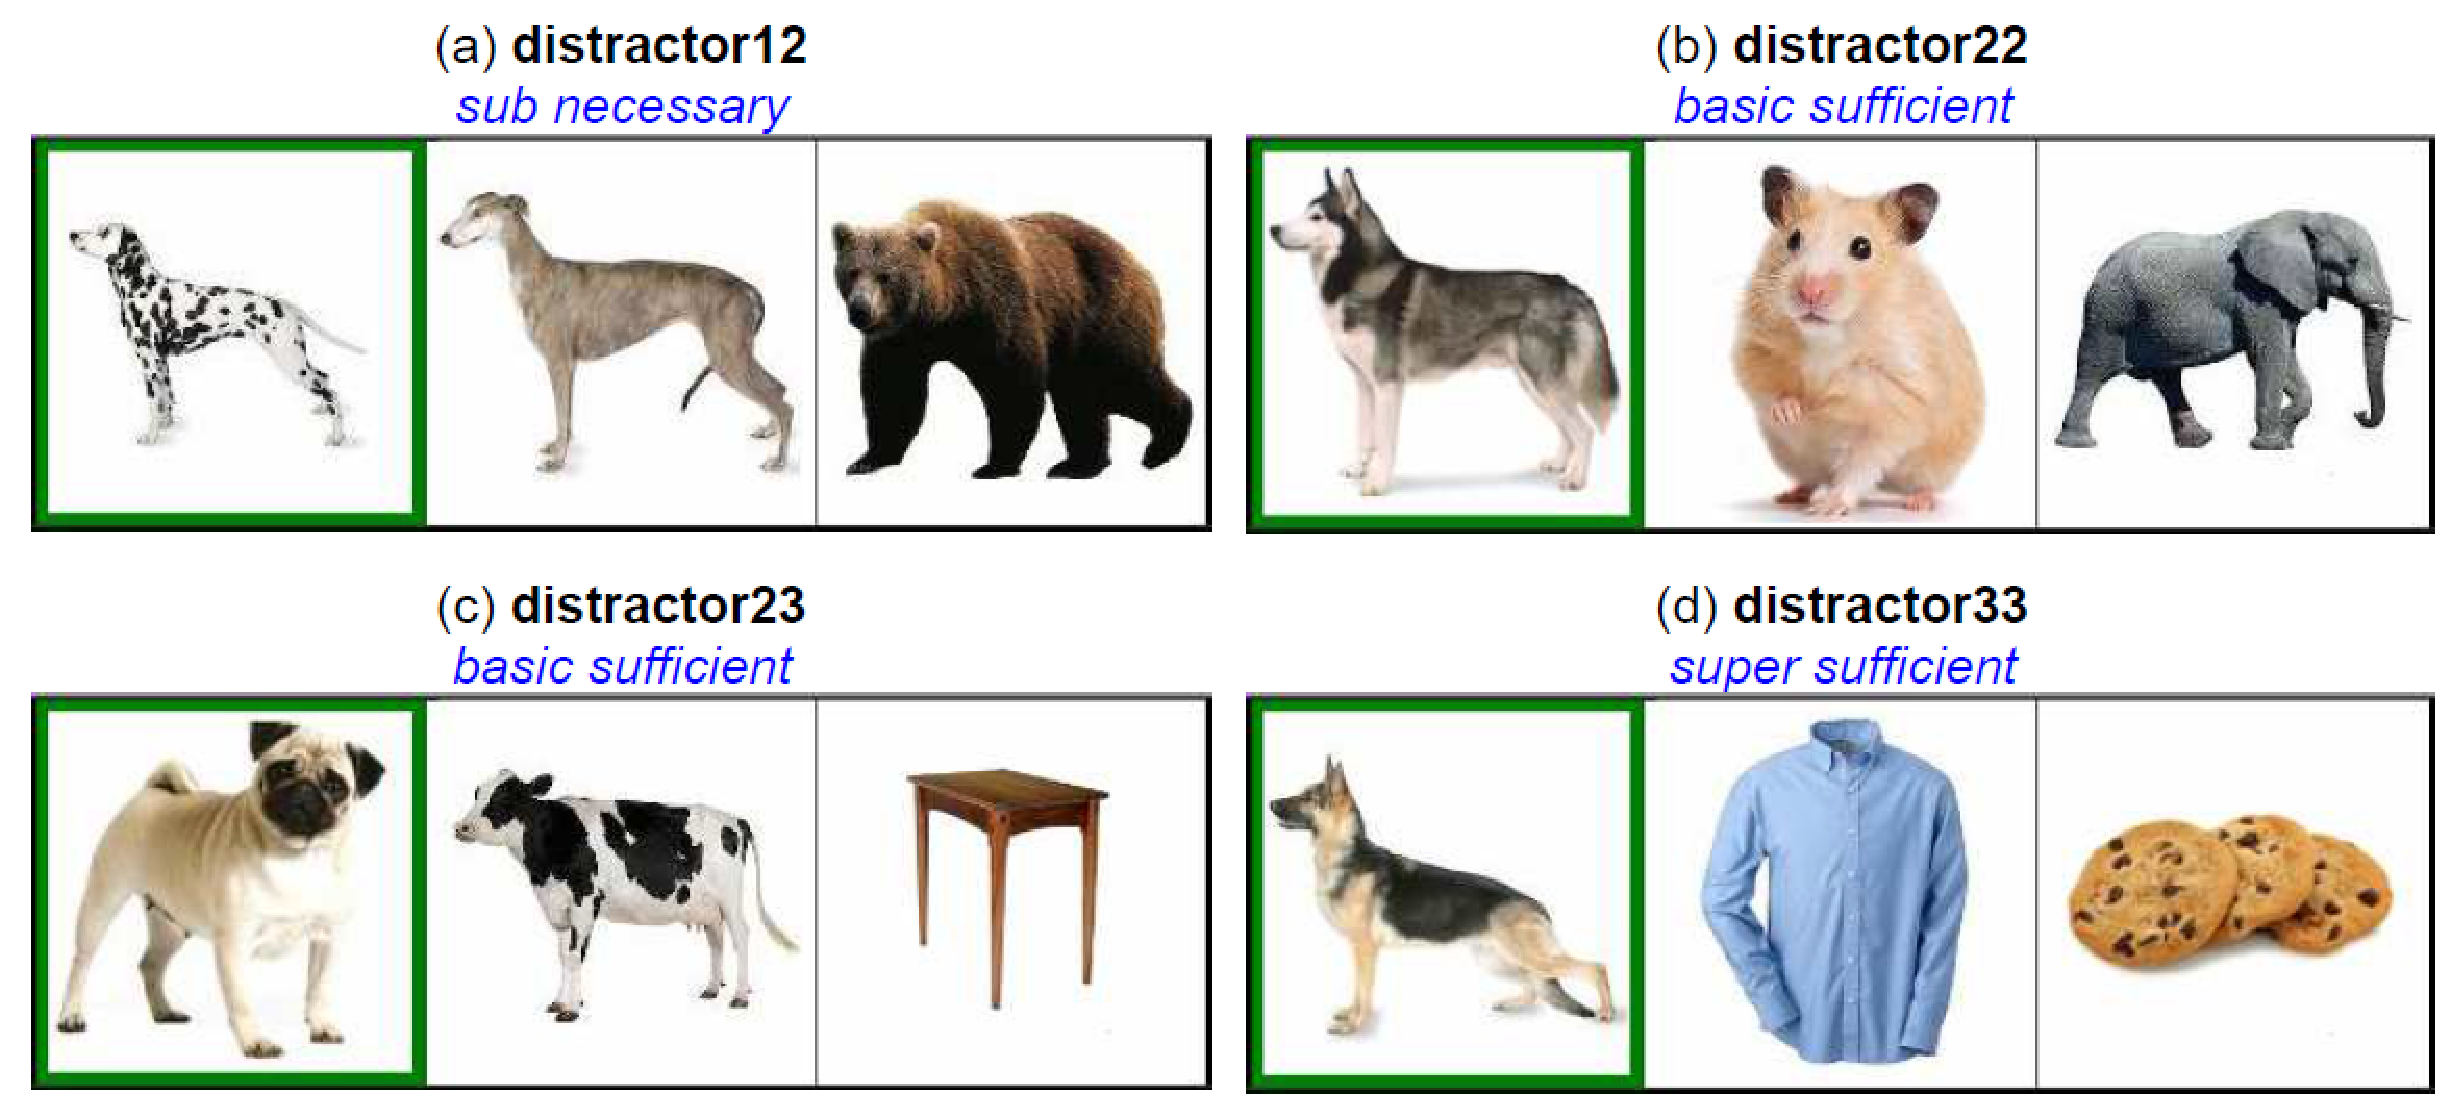
\includegraphics[width=.5\textwidth]{graphs/design}
\caption{Notation used for the four conditions, exemplified by the \textit{dog} domain. The target can be identified by a green box surrounding it and is in the case of the \textit{dog} domain always a type of dog; the types of distractors differ with condition: in the  \textbf{distractor12} condition, a distractor of the same basic level as the target (i.e. a distractor class 1) and a distractor of the same super level as the target (i.e. a distractor class 2) is presented. In \textbf{distractor22}, both distractors are class 2 distracors. In \textbf{distractor23}, one distractor is a class 2 distractor and the other is an artifact which neither shares the basic level nor super level with the target (i.e. a distractor class 3). Finally, there are two class 3 distractors in \textbf{distractor33}.}
\label{fig:design}
\end{figure}

\paragraph{\bf Procedure}
Pairs of participants were connected through a real-time multi-player interface \cite{Hawkins15_RealTimeWebExperiments}. Subjects participated in pairs, with one member of each pair assigned the speaker role and the other to the listener role. Participants kept their allotted roles for the entire experiment. 
The setup for both the speaker and the listener is shown in Fig. 2. Each saw the same set of three images, however participants were informed that image placement would be (and in fact was) different for the speaker and the listener. The target object was identified by a green square surrounding it for the speaker (but not listener). There was a chatbox in which speaker and listener could send text messages to each other. The task was for the speaker to tell the listener which one of the objects is the target, and for the listener in turn to select the right object based on the information provided by the speaker. 

\begin{figure}[ht!]
\centering
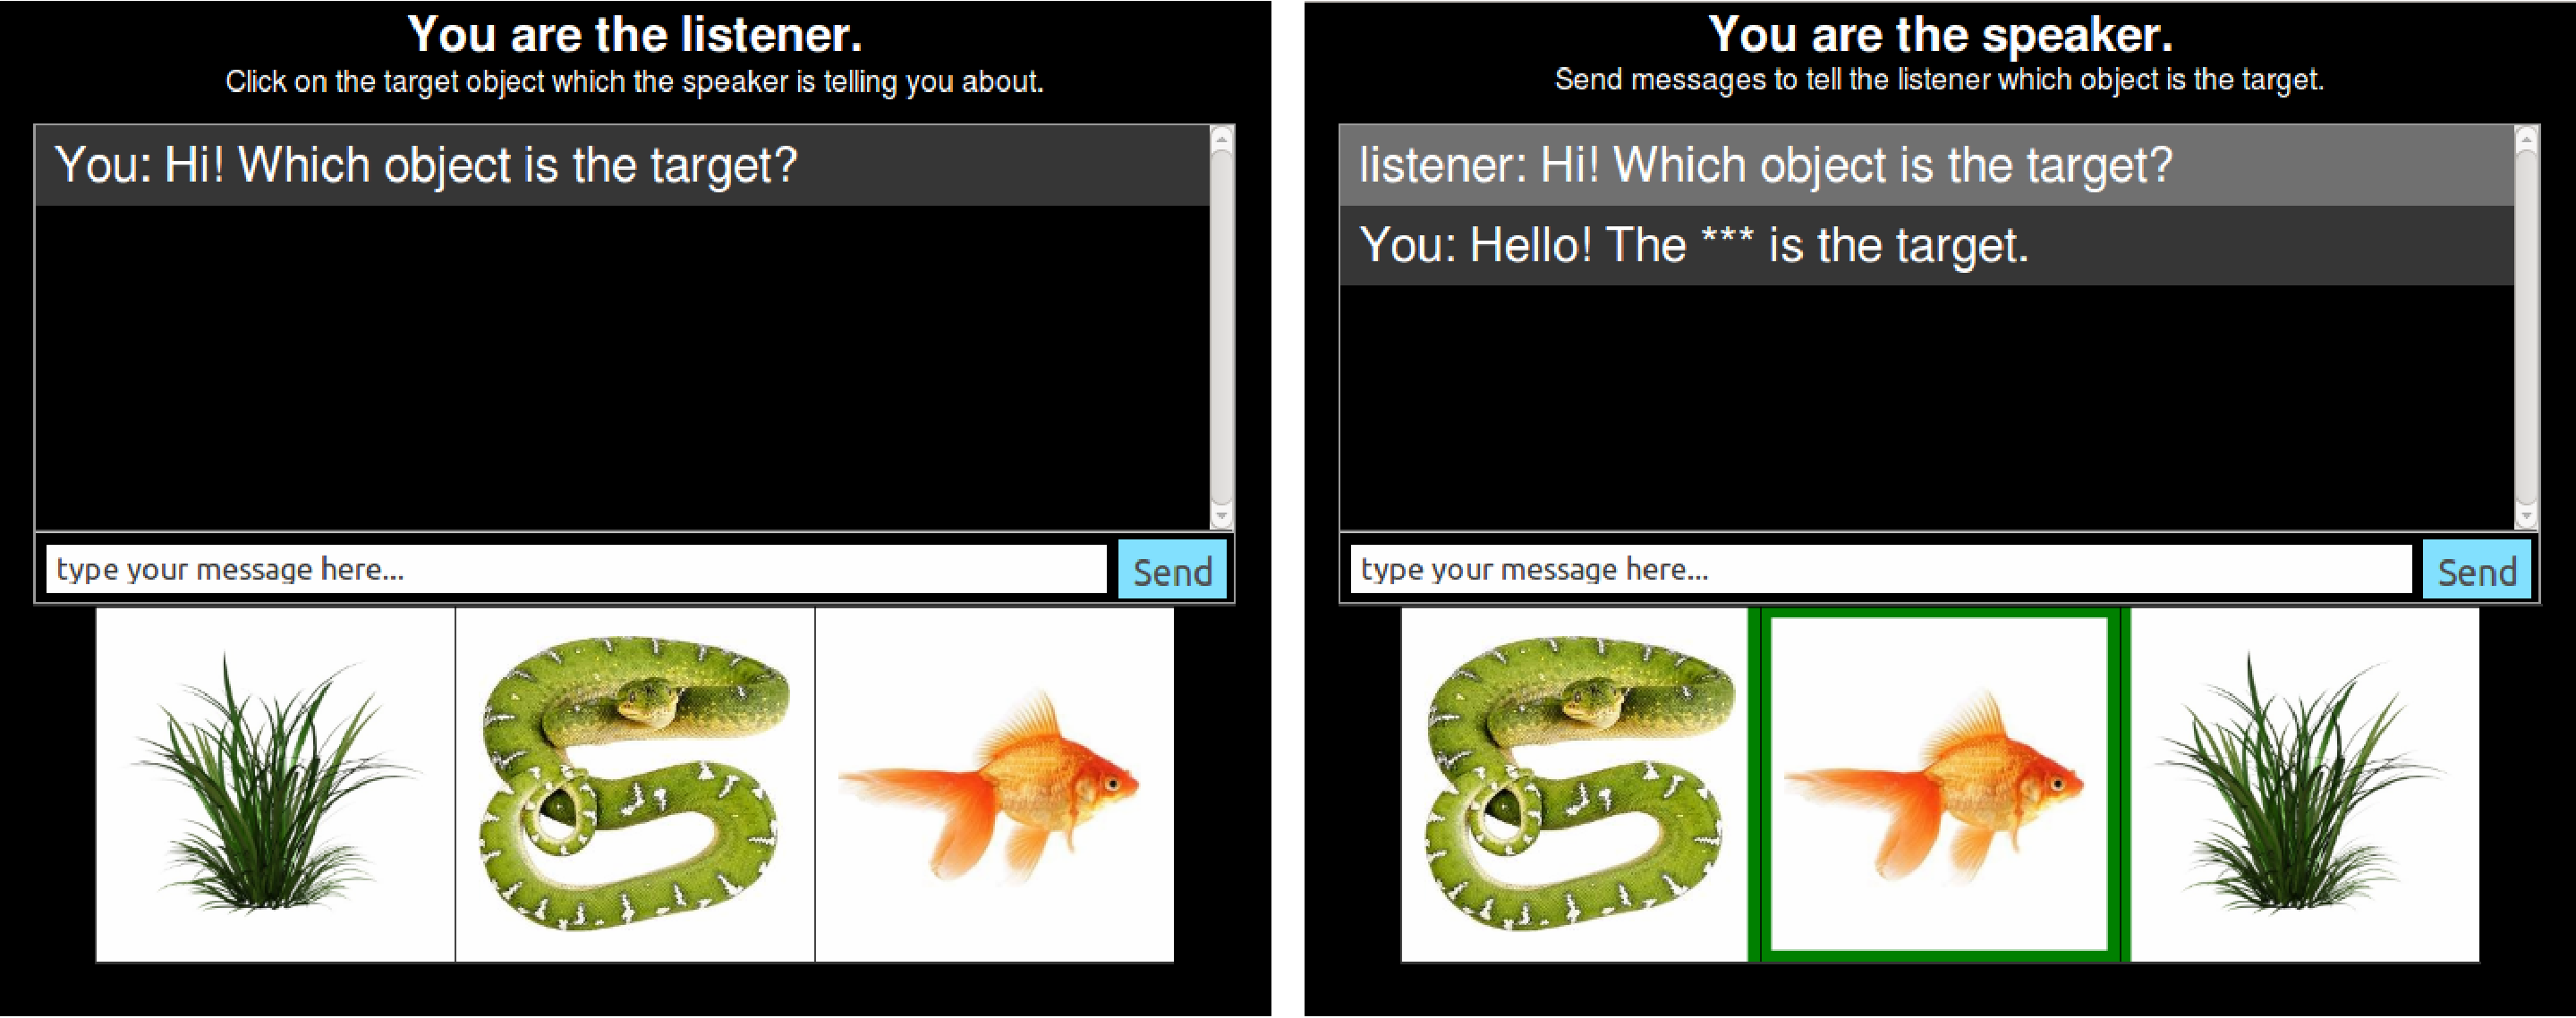
\includegraphics[width=.5\textwidth]{graphs/procedure}
\caption{Screenshots from speaker' and listener' points of view, showing role names and short task descriptions, the chatbox used for communication and a display of three pictures of objects, one of which the speaker could identify as a target by a green box surrounding it.}
\label{fig:procedure}
\end{figure}

\paragraph{\bf Annotation}
Trials on which the listener selected the wrong referent were excluded from the analysis, which led to the elimination of 1.1\% of trials.
 
Speakers' and listeners' messages were first parsed automatically; the referential expression used by the speaker was extracted for each trial and checked for whether it contained the current target's correct sub, basic or super level term using a simple grep search. In this way, 66.2\% of trials were labelled as mentioning a pre-coded level of reference. In the next step, utterances were checked manually to determine whether they contained a correct level of reference term which was not detected by the parsing algorithm due to typos or grammatical modification of the expression. In this way, meaning-equivalent alternatives such as ``doggie'' for ``dog'',  or contractions such as ``gummi'',``gummies'' and ``bears'' for ``gummy bears'' were counted as containing a level of reference term. By this means another 13.8\% of trials were included in the analysis. A total of 10.0\% of correct trials were excluded, because the utterance consisted of an attribute of the superclass (``the living thing'' for ``animal''), of the basic level (``can fly'' for ``bird''), of the subcategory (``barks'' for ``dog'') or of the  particular instance (``the thing facing left'') was mentioned rather than a level of reference term. These kinds of attributes were also sometimes mentioned additionally to the level of reference term in the trials which were included in the analysis, that is, 4.0\% of sub level terms, 12.6\% of basic level terms, and 46.2\% of super level terms contained an additional modifier. By making use of attributes,  speakers could generate unambiguous referential expressions despite using a level of reference which would by itself be insufficient for disambiguation, e.g. by referring to a dalmatian as a ``spotted dog'' (in the context of another dog being present, for instance a pug which is not spotted). Furthermore, 0,5\% of trials mentioned two different levels of reference, in this case the more specific level of reference was counted as being mentioned in this trial. Additional processing also established the number of correct trials where a determiner (``the'' or ``a''/``an'') or an indefinite referent such as ``one'', ``thing'' or ``object'' was used, how many correct trials consisted of complete sentences and the number of correct trials where level of reference terms were contracted (namely 2.7\%, 0.9\%, 1.0\% and 5.3\% respectively). \jd{do we need the last bit of info, since we don't actually go on to do anything with it?}


\subsection{\bf Results}

Proportions of sub, basic, and super level utterance choices in the different conditions are shown in \figref{fig:qualitativemodel} alongside model predictions. The sub level term was preferred where it was necessary for unambiguous referent identification, i.e., when a distractor of the same basic level category as the target was present in the scene (condition distr12, e.g., target: dalmatian, distractor: greyhound). Where it was not necessary (i.e., when there was no other object of the same basic level category present, as in conditions distr22, distr23 and distr33), there was a clear preference for the basic level term. The super level term was strongly dispreferred overall, though it was used on some trials, especially where informativeness constraints on utterance choice were weakest (condition distr33). 
%
%\begin{figure}[ht!]
%\centering
%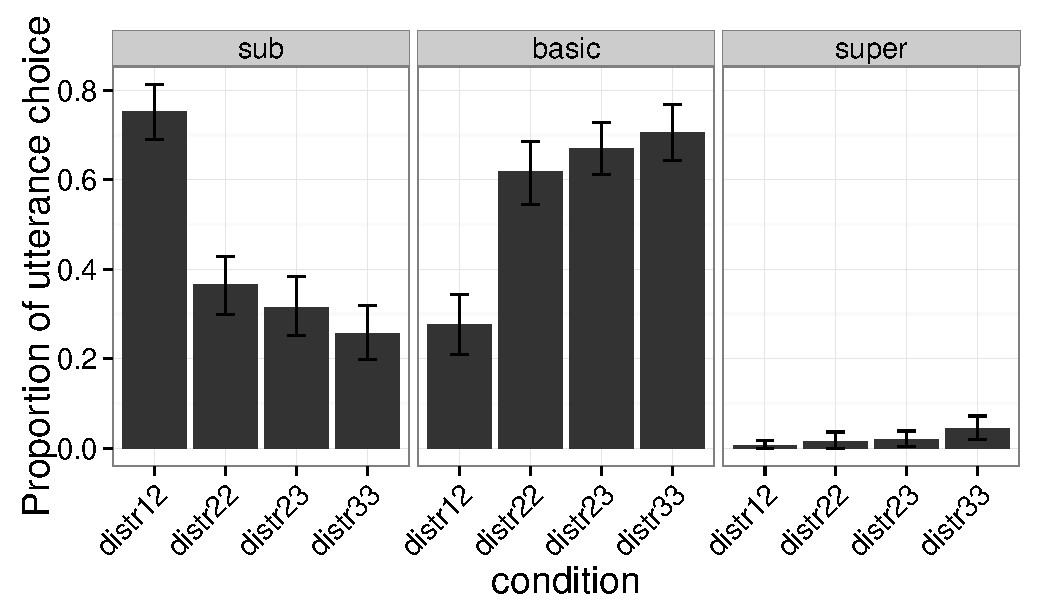
\includegraphics[width=.5\textwidth]{graphs/results-collapsed}
%\caption{Proportion of utterance choice by condition. Error bars indicate bootstrapped 95\% confidence intervals.}
%\label{fig:results1}
%\end{figure}

To test for the independent effects of informativeness, length, frequency, and typicality on sub level mention, we conducted a mixed effects logistic regression. Frequency was coded as the difference between the sub and the basic level's log frequency, as extracted from the Google Books Ngram English corpus ranging from 1960 to 2008. Length was coded as the ratio of the sub to the basic level's length.\footnote{We used the mean empirical lengths in characters of the utterances participants produced at the sub and basic level. For example, the minivan, when referred to at the subcategory level, was sometimes called "minivan" and sometimes "van", leading to a mean empirical length of 5.64. This is the value that was used, rather than 7, the length of "minivan". Using the lengths of the intended labels rather than the empirical means did not change the results qualitatively.} That is, a higher frequency difference indicates a \emph{lower} cost for the sub level term compared to the basic level, while a higher length ratio reflects a \emph{higher} cost for the sub level term compared to the basic level. 

Typicality estimates were obtained in a separate norming study. Due to the large number of possible combinations of objects, we only collected norms for certain combinations of objects and labels: for each target (e.g., dalmatian), we collected norms for how typical it is when referred to at the sub (``dalmatian''), basic (``dog''), and super (``animal'') level. For each distractor of a different superclass (\emph{distdiffsuper}, e.g., basketball in the dalmatian context) we collected norms for how typical it is when referred to with the superclass label (``animal'') and assume lowest typicality otherwise (when referred to as ``dalmatian" or ``dog"). Finally, for each distractor of the same superclass (\emph{distsamesuper}, e.g., kitten), we collected norms for how typical it is when referred to at the sub, basic, and superclass level. This resulted in the following distribution of norms:  \emph{target-sub} (36), \emph{target-basic} (36), \emph{target-super} (36), \emph{distdiffsuper-super} (168), \emph{distsamesuper-sub} (331), \emph{distsamesuper-basic} (93), and \emph{distsamesuper-super} (45). On each trial, participants saw an object image (the same images used in Exp.~1) with the question ``How typical is this for X?'', where X was replaced with the label to be tested. They then adjusted a slider bar ranging from \emph{not at all typical} to \emph{very typical}. Each participant provided typicality ratings for 7 \emph{target}, 10 \emph{dist-diffsuper}, and 28 \emph{dist-samesuper} cases (randomly sampled from the total set of items). Each case received between 6 and 27 ratings. In the regression analysis, typicality was coded as the ratio of the target's sub to basic level label typicality. That is, the higher the ratio, the more typical the object was for the sub label compared to the basic level; or in other words, a higher ratio indicates that the object was relatively atypical for the basic label compared to the sub label. \jd{should we add a separate section for reporting the typicality norming experiment?}

Condition was coded as a three-level factor: \emph{sub necessary}, \emph{basic sufficient}, and \emph{super sufficient}, where distr22 and distr23 were collapsed into \emph{basic sufficient}. Condition was Helmert-coded: two contrasts over the three condition levels were included in the model, comparing each level against the mean of the remaining levels (in order: \emph{sub necessary}, \emph{basic sufficient}, \emph{super sufficient}). This allowed us to determine whether the probability of type mention  for neighboring conditions suggested by \figref{fig:qualitativemodel} were significantly different from each other.\footnote{Adding terms that code the ratio of the sub vs super level frequency and length did not lead to an improvement of model fit.} The model included random by-speaker and by-domain intercepts. 



A model summary is shown in \tableref{tab:modelresults}. The log odds of mentioning the sub level term was greater in the \emph{sub necessary} condition than in either of the other two conditions, and greater in the \emph{basic sufficient} condition than in the \emph{super sufficient} condition, suggesting that the contextual informativeness of the sub level mention has a gradient effect on utterance choice. There was also a main effect of typicality, such that the sub level term was preferred for objects that were more typical for the sub level compared to the basic level  description (see \figref{fig:typicalityeffect}). In addition, there was a main effect of length, such that as the length of the sub level term increased compared to the basic level term (``chihuahua''/``dog'' vs.~``pug''/``dog''), the sub level term was dispreferred (i.e., ``chihuahua'' is dispreferred compared to ``pug'', see \figref{fig:lengtheffect}). Finally, while there was no main effect of frequency, we observed a significant length by frequency interaction (visualized in \figref{fig:lengthfreqinteraction}), such that there was a frequency effect for the relatively shorter but not the relatively longer sub-level cases: for shorter sub level terms, relatively high-frequency sub level terms were more likely to be used than relatively low-frequency sub level terms. 



\begin{table}[!tbp]
\caption{Mixed effects model summary.}
\begin{center}
\begin{tabular}{lrrl}
\toprule
\multicolumn{1}{l}{}&\multicolumn{1}{c}{Coef $\beta$}&\multicolumn{1}{c}{SE($\beta$)}&\multicolumn{1}{c}{$p$}\tabularnewline
\midrule
Intercept&$-0.30$&$0.35$&\textgreater0.4\tabularnewline
Condition sub.vs.rest&$ 2.46$&$0.24$&\textbf{\textless.0001}\tabularnewline
Condition basic.vs.super&$ 0.52$&$0.23$&\textbf{\textless.05}\tabularnewline
Length&$-0.52$&$0.14$&\textbf{\textless.001}\tabularnewline
Frequency&$-0.02$&$0.08$&\textgreater0.78\tabularnewline
Typicality&$ 4.17$&$0.84$&\textbf{\textless.0001}\tabularnewline
Length:Frequency&$-0.30$&$0.11$&\textbf{\textless.01}\tabularnewline
\bottomrule
\end{tabular}\end{center}
\label{tab:modelresults}
\end{table}


\begin{figure}[ht!]
\centering
%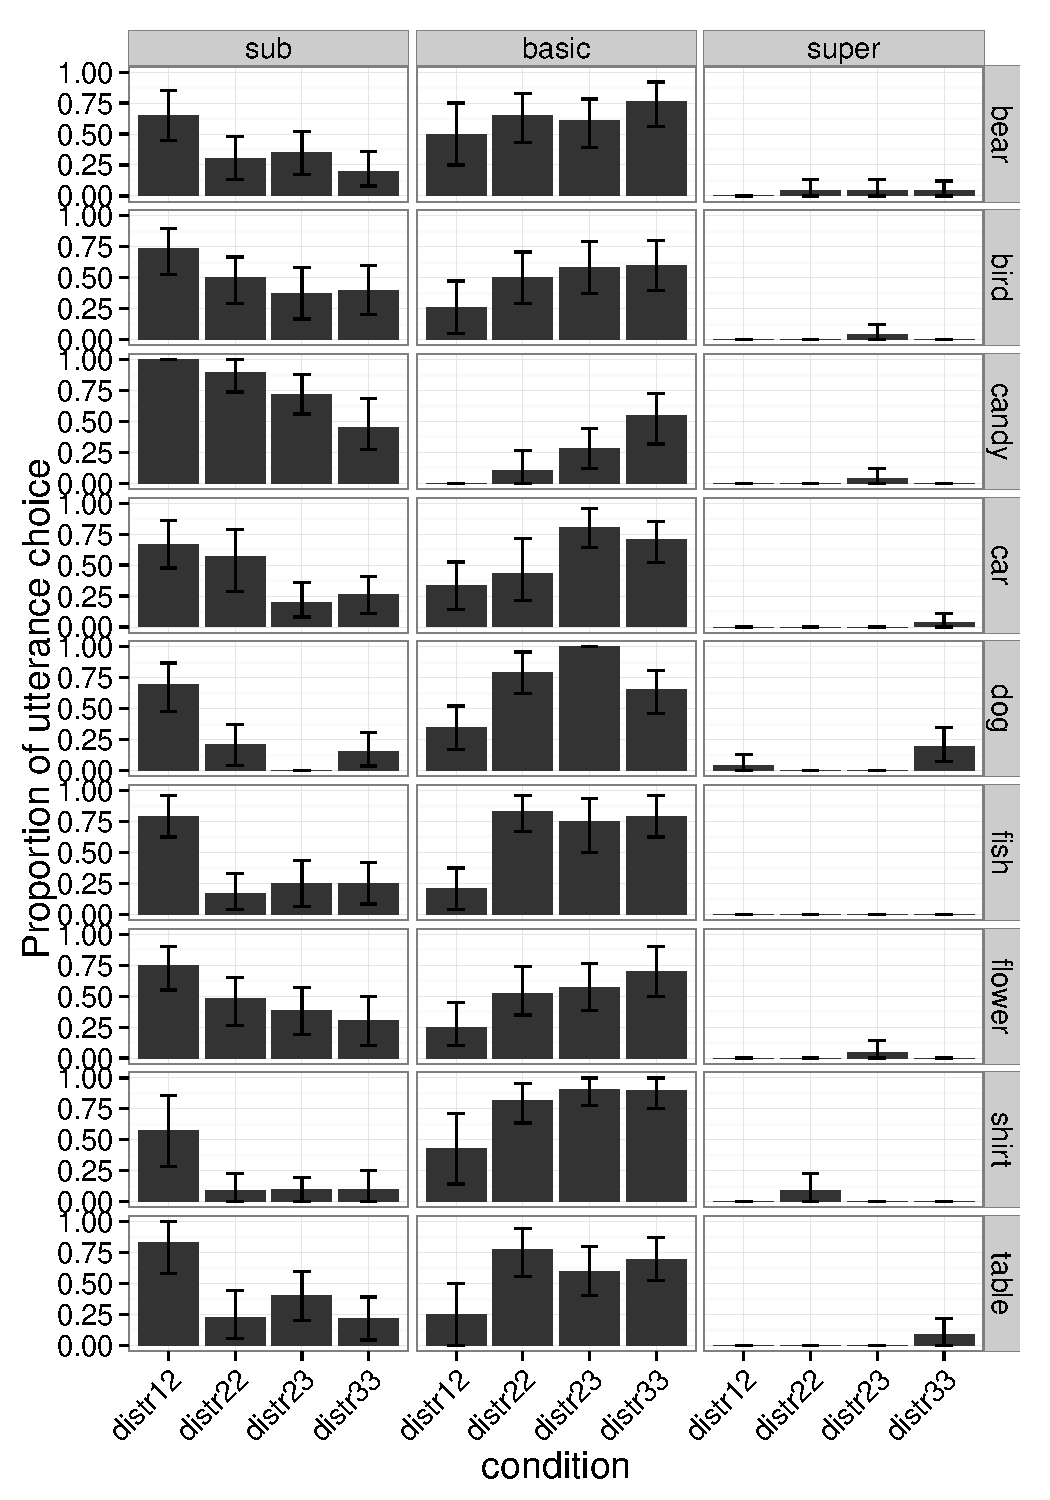
\includegraphics[width=.5\textwidth]{graphs/results-bydomain}
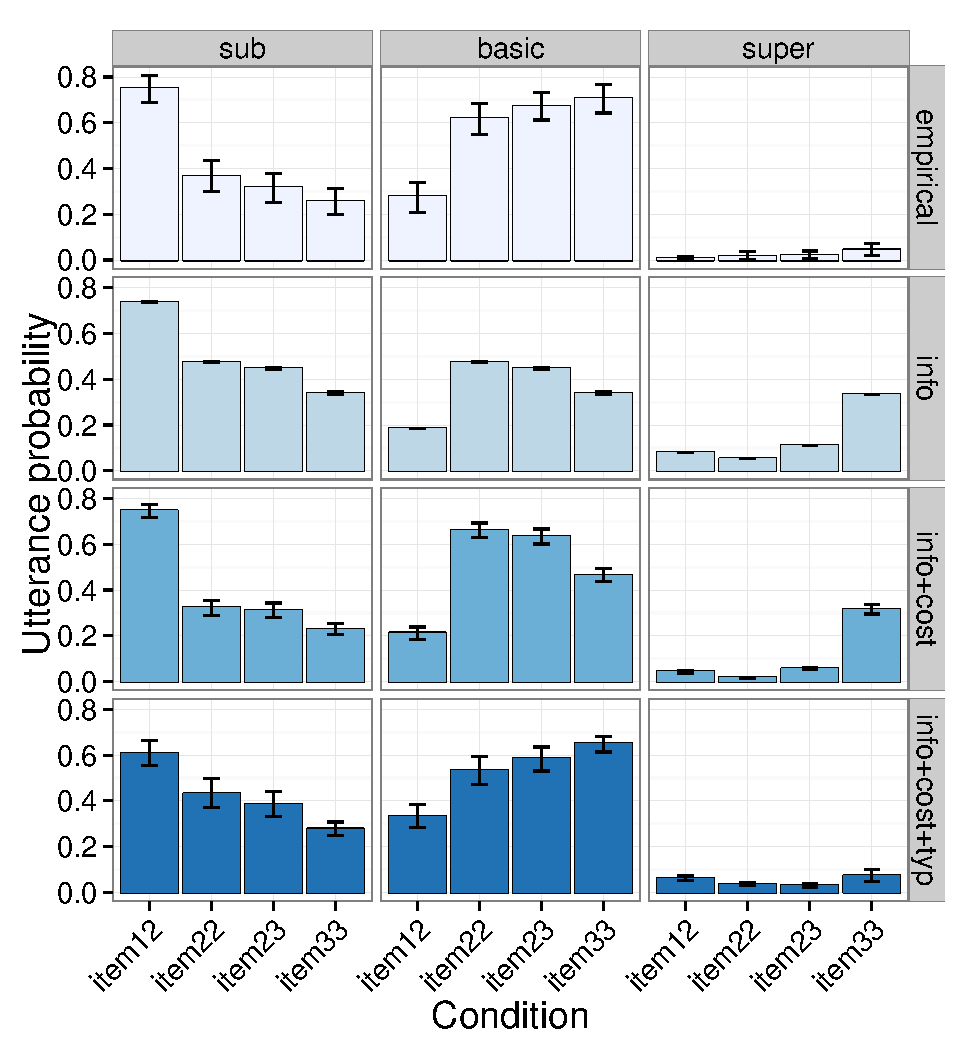
\includegraphics[width=.5\textwidth]{graphs/collapsed-pattern}
\caption{Empirical results and model predictions (increasingly complex from top to bottom) by condition, collapsed across targets and domains. Error bars indicate bootstrapped 95\% confidence intervals.}
\label{fig:qualitativemodel}
\end{figure}

\begin{figure}[ht!]
\centering
%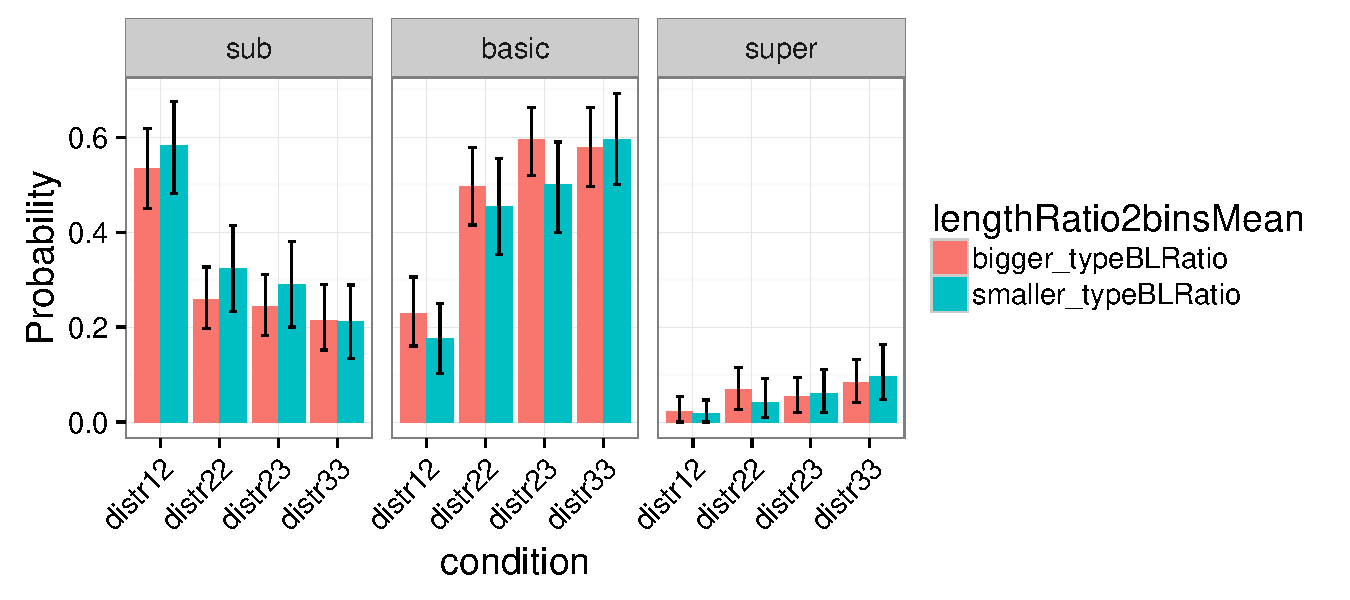
\includegraphics[width=.5\textwidth]{graphs/lengthRatio}
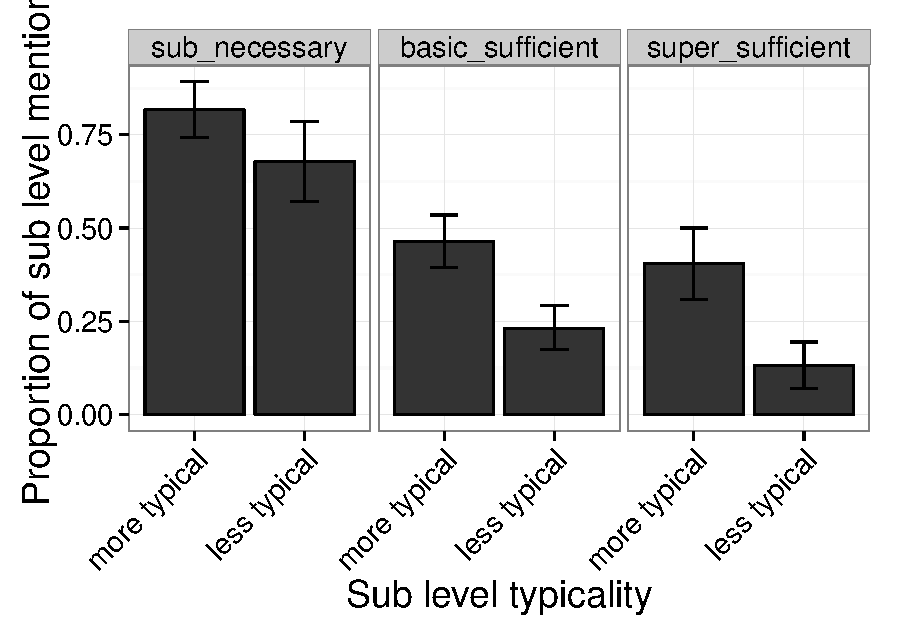
\includegraphics[width=.5\textwidth]{graphs/typicality-effect}
\caption{Probability of using sub, basic and super level terms when the target object was relatively more [1.06,1.91) or less (.88,1.06] typical for the sub compared to the basic level term .}
 \label{fig:typicalityeffect}
\end{figure}


\begin{figure}[ht!]
\centering
%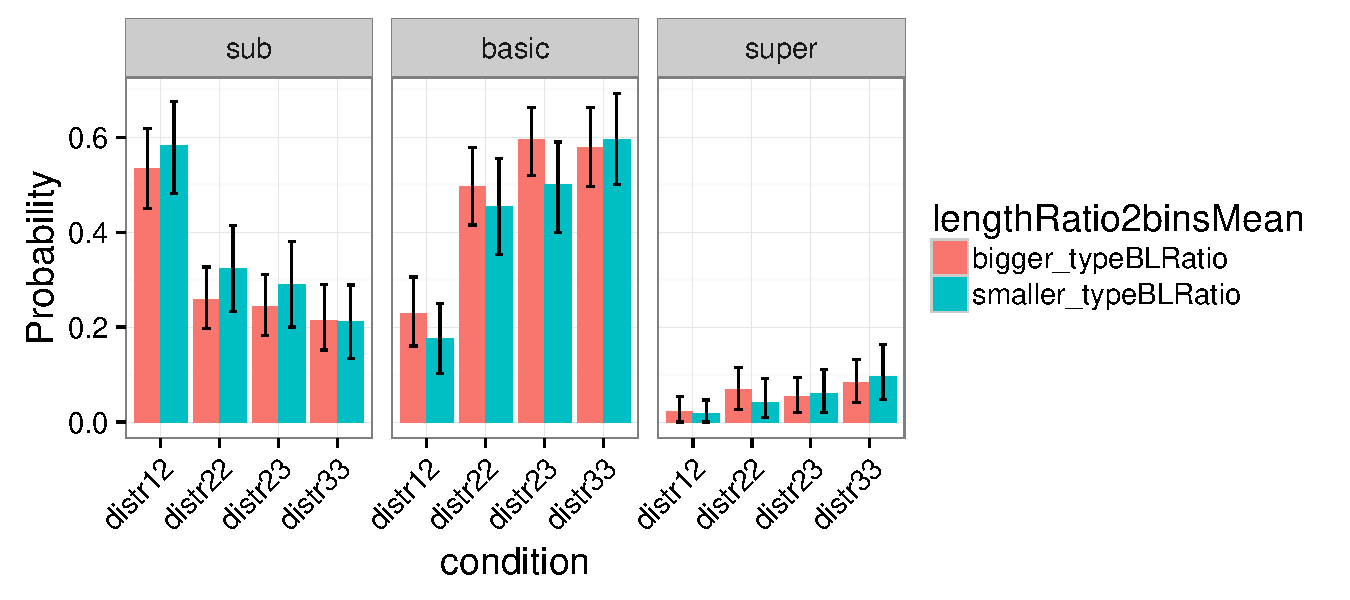
\includegraphics[width=.5\textwidth]{graphs/lengthRatio}
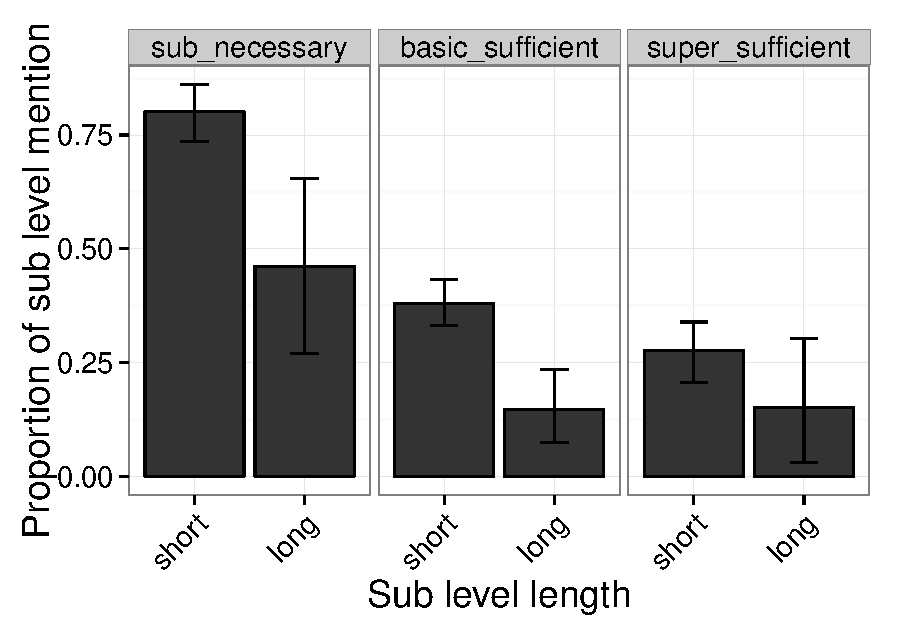
\includegraphics[width=.5\textwidth]{graphs/length-effect}
\caption{Probability of using sub, basic and super level terms when the sub  length is relatively short (.67,2] or long [2,4.67) compared to the basic level term length.}
 \label{fig:lengtheffect}
\end{figure}



\begin{figure}[ht!]
\centering
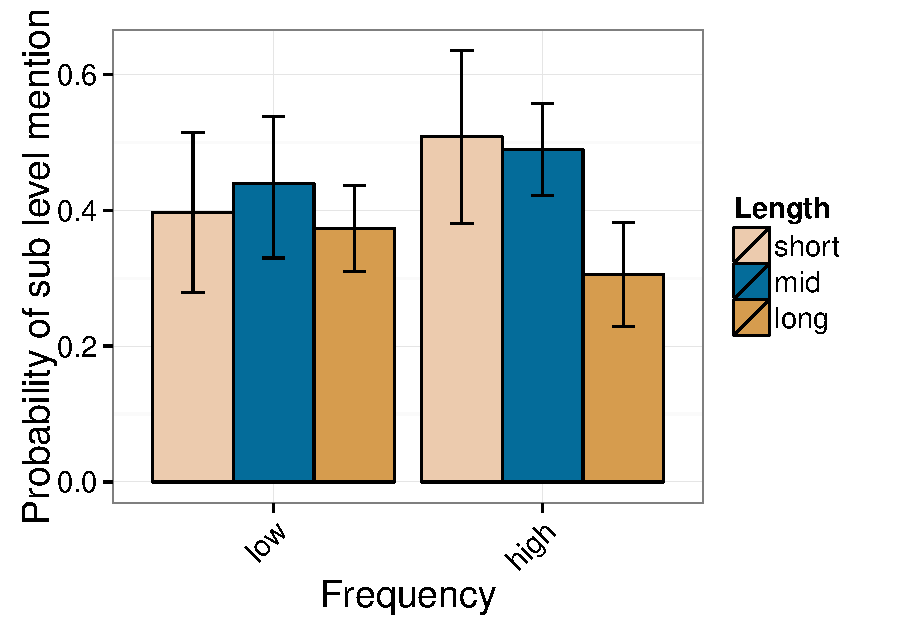
\includegraphics[width=.5\textwidth]{graphs/freq-length-interaction}
\caption{Proportion of sub level mentions  as a function of the sub level term's relative length and frequency compared to the basic level. Length bins reflect the sub/basic length ratio intervals (0, 1] (short), (1, 2] (mid), (2, 4.67] (long). Frequency bins reflect the sub/basic log frequency difference intervals (-11.2,-5.19] (low), (-5.19,-0.65] (high).}
\label{fig:lengthfreqinteraction}
\end{figure}


Unsurprisingly, there was also significant by-participant and by-domain variation in the log odds of sub level mention. %\figref{fig:bigscatterplot} shows the by-domain variation in utterance choice. 
For instance, mentioning the subclass over the basic level term was preferred more in some domains (e.g. in the ``candy'' domain) than in others. Likewise, some domains had a greater preference for basic level terms (e.g. the ``shirt'' domain). Using the superclass term also ranged from hardly being observable (e.g. the ``flower'' domain) to being used more frequently (e.g. in the ``bird'' domain). Nevertheless, mentioning the sublevel category was always the most frequent choice of utterance in the case where a distractor of the same basic level was displayed. Furthermore, the sublevel term was always mentioned most frequently and the basic level least frequently in just this condition, compared to the other three conditions.



These results suggest that the choice of level of reference depends in a gradient manner on both the informativeness of the reference level as well as on the fit of the object to a specific label due to typicality and the cost of the corresponding utterance (both in terms of length and frequency) compared to the alternative utterances.




\section{\bf Modeling level of reference}

%To show that we can account for these context effects purely through communicative pressures, we formulated a simple probabilistic model of basic-level reference. 
We formulated a probabilistic model of reference level selection that integrates contextual informativity, utterance cost, and typicality.
As in earlier Rational Speech Act (RSA) models \cite{frank2012, goodmanstuhlmueller2013}, the speaker seeks to be informative with respect to an internal model of a literal listener. This listener updates her beliefs to rule out possible worlds that are inconsistent with the meaning of the speaker's utterance. Rather than assuming that words have deterministic truth conditions, as has usually been done in the past, we account for typicality by allowing each label a graded meaning. For instance, the word ``dog'' describes a dalmatian better than a grizzly bear, but it also describes a grizzly bear better than a tennis ball.
The speaker also seeks to be parsimonious: the speaker utility includes both informativity and word cost; cost includes both length and frequency.

Formally, we start by specifying a literal listener $L_0$ who hears a word $l$ at a particular level of reference  in the context of some set of objects $\mathcal{O}$ and forms a distribution over the referenced object, $o \in \mathcal{O}$ : 
$$P_{L_0}(o | l) \propto \denote{l}(o).$$
Here $\denote{l}(o)$ is the lexical meaning of the word $l$ when applied to object $o$. We take this to be a real number indicating the degree of acceptability or typicality of object $o$ for category $l$, for which we use the empirical typicality norms elicited earlier. \ndg{fix up wrt norms refernce}

Next, we specify a speaker $S_1$ who intends to refer to a particular object $o \in \mathcal{O}$ and chooses among possible words $l \in \ell(o)$: 
$$P_{S_1}(l | o) \propto \exp(\lambda \ln P_{L_0}(o | l) + \beta_f \hat{c}_f  + \beta_l \hat{c}_l + \beta_{fl} \hat{c}_{fl} )$$
Thus the speaker chooses labels in a way that is influenced by informativity of the label for the literal listener ($\ln P_{L_0}(o | l)$), the frequency cost ($\hat{c}_f$), and the length cost ($\hat{c}_l$).
Length cost $c_l$ is defined as the mean number of characters used to refer at that level empirically as obtained in the previously reported experiment. For example, the gummy bears were frequently referred to as ``gummies'', leading to a mean word length of 8.9. Frequency cost $c_f$ is estimated using the log probability of occurring in the Google Books corpus from 1960 to the present. In addition, given the significant interaction between length and frequency observed in the regression analysis, we included a multiplicative cost term $c_fl$, which was \jd{integrated how exactly?} \ndg{are the length and freq defined in the previous section? }
The relative importance of these three factors is determined by three parameters that were fit to the data.
%where $U_{cost}(l_j)$ is the label cost function and $\alpha$ is an optimality parameter\footnote{$\alpha = 1$ corresponds to a soft-max decision rule, and $\alpha \rightarrow \infty$ corresponds to a optimal hard-max decision rule.}. \ndg{is there a parameter for relative importance of informativity and cost?}

%Finally, we must specify the the lexical meaning function $\denote{l}(o_i)$ and the cost function $U_{cost}(l_j)$. 
%\red{rdh: we'll probably want to write down how we compute length and frequency earlier, since some results depend on them.}
%We measure label cost as the linear combination of two components: length and frequency. Length cost $c_l$ is defined as the number of characters in the label, and frequency cost $c_f$ is estimated using the log probability of occurring in the Google Books corpus from 1960 to the present. To trade these two measures off against one another, we compute normalized scores $\hat{c}_l \in [0,1]$ and $\hat{c}_f \in [0,1]$ by subtracting the minimum score of all labels used in the experiments and dividing by the range. We then define the label cost of $l_j$ to be $$U_{cost}(l_j) = w\hat{c}_f - (1-w)\hat{c}_l$$ where $w \in [0,1]$ is a parameter controlling the tradeoff between length and frequency.

Parameters were fit to maximize the correlation of model predictions and by-target empirical proportions of sub, basic, and super level term use by condition. A total of 432 data points were fit (four targets per domain for nine domains, and for each target, three utterance choices in four conditions). The best parameter values are listed in \tableref{tab:bestparams} (bottom row). 

\begin{table}
\caption{Maximal correlation and best model parameters, fit to the empirical by-target by-utterance and by-condition proportion, for increasingly complex models.}
\begin{center}
	\begin{tabular}{l l l l l l}
	\toprule
	Model & max $r$ & $\lambda$ & $\beta_f$ & $\beta_l$ & $\beta_{fl}$\\
	\midrule
	info & .6 &  & NA & NA & NA\\
	info + cost  & .7 & & & & \\
	info + cost + typicality  & .75 & & & & \\
	\bottomrule
	\end{tabular}	
\end{center}
\label{tab:bestparams}
\end{table}

On the by-target level, the model achieves a correlation of $r = .75$ by rating informativeness relatively strongly ($\lambda$ = \red{fix}), the length cost term somewhat more weakly ($\beta_l =$\red{fix}), and the frequency and frequency-by-length interaction term yet more weakly ($\beta_f$ = \red{fix} and $\beta_{fl} =$ \red{fix}).

In order to ascertain whether the cost and typicality terms were indeed contributing to the explanatory power of the model, we compared the model against simpler versions: one that included only an informativeness term (\tableref{fig:bestparams}, first row) and one that included informativeness and the cost terms but no typicality (\tableref{tab:bestparams}, second row). Both cost and typicality add explanatory value to the model.

\jd{add the bit about collapsing across targets and then across domains}

\ndg{MODEL RESULTS AND ANALYSIS!!}


\section{\bf Discussion and conclusion}

-summary paragraph- 

\ndg{things to say: we got naturalistic data of nominal reference. this was affected by cost (length), context, and typicality. these factors fit naturally into an RSA model. this predicts basic-level bias without building it in, and interactions between these factors. future work will need to explore: the item effects where perhaps visual salience plays a role (or something else?); the interaction of nominal and modifier choice; the role of typicality in RSA models. connect to rosch, the dutch guys, naomi's student.}

Length and frequency of utterances and their alternatives play an important role in determining the type of referential expression used. Shorter labels are preferred, even more so when the sub level term is more frequent. [Something about typicality] However, length and frequency (and typicality???) do not account completely (?) for utterance choice...

Thus, there seems to be something else about basic levels that makes them so favorable. Rosch et al. (1976) characterize basic level terms as carrying the most information, possessing the highest category cue validity, being most differentiable from each other and being the most inclusive level of abstraction categories for which a concrete image of the category as a whole can be formed. However, the bounds as to what is considered a basic level term are not always completely clear. For instance, ``fish'' was used as a basic level category in the current study and subordinate terms thereof (e.g. ``clownfish'' and ``goldfish'') seem clearly to be types or sublevel terms, but ``shark'' on the other hand seems intuitively to be more of a basic level itself, giving rise to its own sublevel terms (e.g. ``Great white shark'') (?or is this just my intuition?) (I though I read something along these lines somewhere else too, I need to have a look at the lit again to check this and then explain a little more ...)

Furthermore, some specific items in the study were referred to by their sublevel term exceptionally often (specifically ``eagle'', which was referred to with the sub level term ``eagle'' in 91\% of trials). Perhaps this is due to the ``cultural salience'' of ``eagle'', i.e. in American culture the eagle is a very prominent part of world knowledge. And many researchers agree that world knowledge plays an important part in human categorization behavior (e.g. Jolicoeur et al., 1984; Murphy and Medin, 1985) and is thus also essential in choosing a level of reference. For instance, Tanaka and Taylor (1991) demonstrated that domain-specific ``expert'' knowledge can diminish the preference effect of the basic level to an extent that subordinate level terms are chosen as often as basic level terms to refer to an object.

Another factor which may contribute to the choice of utterance may be perceptual saliency. Saliency as a major mechanism in cognitive neuroscience is essential for allocating attentional resources and has also been in found to be a factor contributing to utterance choice in other areas of referential expression (Westerbeek et al.). Perhaps this could explain some of the more extreme item effects found in this study. For instance, the ``candy'' domain showed a remarkable preference for the sublevel term. This could possibly be explained by the fact that these pictures of ``gummy bears'', ``jelly beans'', ``M\&M’s'' and ``Skittles'' were extraordinarily colorful and high-contrast, which is specific to each of these sublevel terms, not to candy in general.

[What exactly these other factors are that contribute to the choice of level of reference is to be determined by further research.]

-Concluding paragraph-






\section{\bf Acknowledgments}

This work was supported by ONR grant N00014-13-1-0788 and a James S. McDonnell Foundation Scholar Award to NDG and an SNF Early Postdoc.Mobility Award to JD. RXDH was supported by the Stanford Graduate Fellowship and the National Science Foundation Graduate Research Fellowship under Grant No. DGE-114747.

\small


\bibliographystyle{apacite}

\setlength{\bibleftmargin}{.125in}
\setlength{\bibindent}{-\bibleftmargin}

\bibliography{bibs}


\end{document}